  \documentclass[a4paper,11pt]{jbook}
\usepackage{graphicx}% Include figure files
\usepackage{dcolumn}% Align table columns on decimal point
\usepackage{bm}% bold math
\usepackage{amssymb}
\usepackage{amsmath}
%\usepackage{here}
\def\vecR {\bm {\mathcal {R} } }
\def\R  {\mathcal {R} }
\pagestyle{plain}
\title{磁石振り子シミュレータ\\PEM}
\author{牧野真人}
\date{\number\year 年\number\month 月\number\day 日}
\begin{document}
\maketitle
\tableofcontents 
 %%%%%%%%%%%%%%%%%%%%%%%%%
\chapter{はじめに}
シミュレーションエンジンPEMについての説明をする。
PEMは力学に関してのシミュレーションを行う。
力学のシミュレーションであるから、力$F$を受ける質量$m$の物体が加速度$a$で運動するニュートンの運動方程式
\begin{equation}
ma=F
\end{equation}
が基礎になる。
しかし、PEMでは、回転の運動方程式を中心に解く。
コマ、振り子のように、一様重力場中で一固定点を持った剛体の回転の問題を解く。
特に、剛体は、磁石を持つとして、磁気ダイポールをもっており、外磁場やダイポール同士で相互作用する。

剛体の運動は、オイラー角あるいは、四元数を用いて計算されることが多いがPEMでは、粒子固定の直交座標系$\bm{u}_1,\bm{u}_2,\bm{u}_3$を計算していく。
厳密解を解くなどの場合は、オイラー角は有用であるし、四元数は、分子動力学シミュレーションのような多数の多体問題を解く場合は効率が高い。
一方で、私の感覚であるが、粒子固定の直交座標系で計算する場合は、分かりやすい。
そのため、ここでは、粒子固定の直交座標系を用いる。

さらに、他に見られない特徴として回転微分演算子
\begin{equation}
\vecR =\sum_{i=1,2,3}\bm{u}_i\times\frac{\partial}{\partial \bm{u}_i}
\end{equation}
を用いる。
%%%%%%%%%%%%%%%%%%%%%%%%%%%%%%%%%%
\chapter{記号など}
このマニュアルでは、スカラー量は、通常のフォントで$A$のように書く。
ベクトル、テンソル量は太字で$\bm{x},\bm{B}$のように書く。

基底ベクトルの添字は、$i,j,k,...$でベクトルのデカルト座標での成分はギリシャ文字$\alpha, \beta,\gamma ...$で表すようにする。

たとえば、ベクトル
%%%%%%%%%%%%%%%%%%%%%%%%%%%%%%%%%%
\chapter{理論}
\section{基礎方程式}
図\ref{fig:3_01_system}のように
実験室が基底ベクトル$\bm{e}_x, \bm{e}_y,\bm{e}_z $で記述される空間とする。
ここで、$\bm{e}_i\cdot\bm{e}_j=\delta_{ij}, (i,j=x,y,z)$である。右手系として$\bm{e}_i\times\bm{e}_j=e_{ijk}\bm{e}_k$である。
ある一体の剛体を考える。この剛体は剛体に固定された基底ベクトル$\bm{u}_1,\bm{u}_2,\bm{u}_3$で剛体の方向を定義する。
この場合も$\bm{u}_i\cdot\bm{u}_j=\delta_{ij}, (i,j=1,2,3)$である。
図\ref{fig:3_01_system}の(a)は剛体が剛体の基底ベクトルで表され、同様に、振り子も固定点のまわりで運動する剛体として計算できる。
\begin{figure}[h]
\centering
  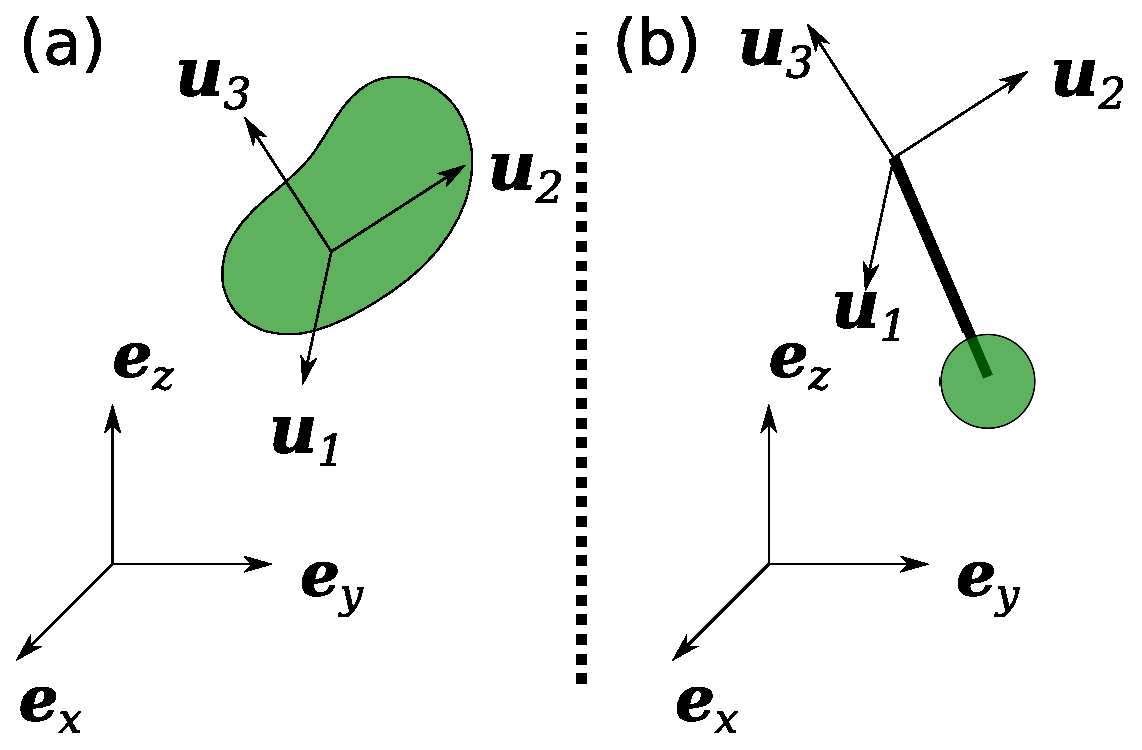
\includegraphics[clip,width=0.8\linewidth]{pict/3_01_system.eps}
  \caption{実験室の基底ベクトル$\bm{e}_x,\bm{e}_y,\bm{e}_z$と剛体固定基底ベクトル$\bm{u}_x,\bm{u}_y,\bm{u}_z$。
  (a)剛体の場合。(b)振り子の場合も剛体として扱う。
  }
  \label{fig:3_01_system}
\end{figure}

トルク$\bm{T}$が与えられた際、角運動量$\bm{L}$の時間微分で与えられる。
\begin{equation}
\frac{d\bm{L}}{dt}=\bm{T}
\label{eq:dLdt}
\end{equation}
また、剛体の角速度$\bm{\omega}$は、剛体の慣性モーメントテンソル$\bm{I}$として
\begin{equation}
\bm{I}\cdot\bm{\omega}=\bm{L}
\end{equation}
となる。
慣性モーメントテンソルは、時間に応じて変化する。
しかし、慣性モーメントテンソルはあらかじめ、粒子に固定した座標系で計算するほうが便利である。
そのため、慣性モーメントテンソルは、次のようにする。
\begin{equation}
\bm{I}(t)=\sum_{i,j=1,2,3}I_{ij}\bm{u}_i(t)\bm{u}_j(t)
\end{equation}
$I_{ij}$は時間に依存しない定数である。粒子固定の座標系で最初に求めておけばよい。
一方で、行列$I_{ij}$の逆行列を$(I^{-1})_{ij}$とすると角速度は
 \begin{equation}
 \bm{\omega}=\sum_{i,j=1,2,3}(I^{-1})_{ij}\bm{L}\cdot\bm{u}_i\bm{u}_j
 \label{eq:omega}
 \end{equation}
 となる。
 これから、
\begin{equation}
\frac{d\bm{u}_i}{dt}=\bm{\omega}\times\bm{u}_i
\label{eq:dudt}
\end{equation}
となる。

トルク$\bm{T}$が与えられると式\eqref{eq:dLdt}より角運動量$\bm{L}$の時間発展を計算する。
次にあらかじめ計算していた慣性モーメントテンソル$I_{ij}$をもとに、式\eqref{eq:omega}より角速度$\bm{\omega}$を計算する。
そして、式\eqref{eq:dudt}より、剛体に固定された基底ベクトル$\bm{u}_i$を計算することで粒子の向きが計算されていく。
このようにして、剛体の運動を計算していくのが、本シミュレータである。
\section{慣性モーメントテンソル}
\subsection{一般の式}
慣性モーメントテンソルは、一様な質量密度$\rho$を持つとして
\begin{equation}
\bm{I}=\rho\int_V\left(r^2\bm{\delta}-\bm{r}\bm{r}\right)dV
\label{eq:inertia_basic}
\end{equation}
と表される。$\bm{r}$は、回転中心からの位置ベクトルで、
$r$は$\bm{r}$の長さである。
積分は、物体の体積$V$に渡って行う体積積分である。

式\eqref{eq:inertia_basic}は、特定の回転中心で評価される。
しかし、任意の回転中心で慣性モーメントテンソル$\bm{I}'$を評価するために、力学の教科書でスタイナーの定理と呼ばれる平行移動の公式は、次のとおりとなる。移動前の慣性モーメントテンソルを$\bm{I}$、質量を$M$、原点から$\bm{r}'$の位置に平行移動すると、平行移動後のテンソル$\bm{I}'$は
\begin{equation}
\bm{I}'=\bm{I}+M\left(r'^2\bm{\delta}-\bm{r}'\bm{r}'\right)
\label{eq:steiner}
\end{equation}
となる。

また、複数の形状がいくつかで、一つの形状が出来ている場合、それぞれの形状での慣性モーメントテンソルを足し合わせれば良い。
ただし、形状が重ねっている場合は、適切ではない。
\subsection{解析解}
PEMに図\ref{fig:3_2_2_shapes}の解析解の慣性モーメントを用いている。
これらを平行移動の公式を用いて、さまざまな形状の振り子、コマなどのシミュレーションが出来る。
\begin{figure}[h]
\centering
  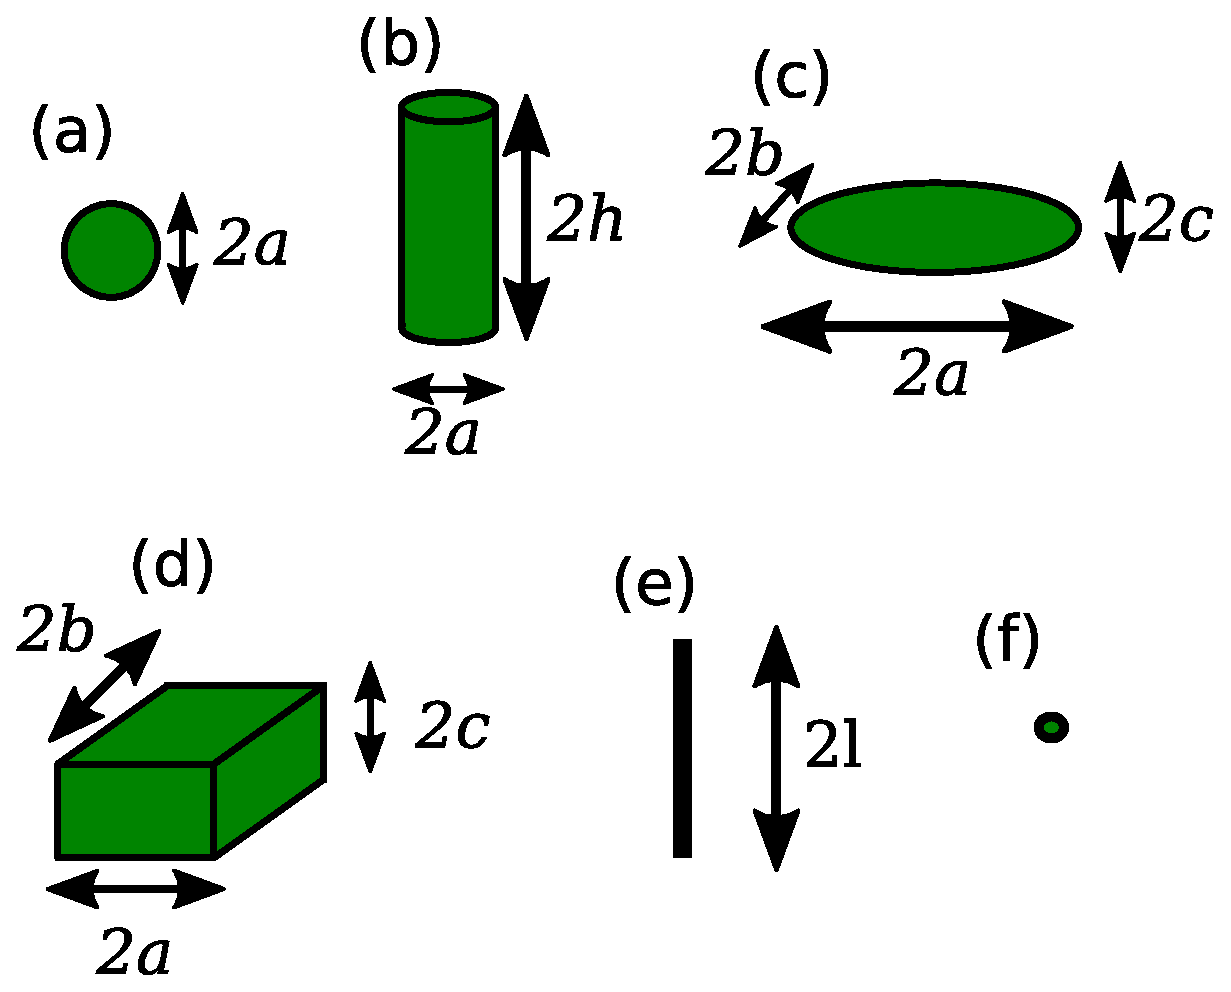
\includegraphics[clip,width=0.8\linewidth]{pict/3_2_2_shapes.eps}
  \caption{さまざまな形状。(a)半径$a$の球。(b)底面の半径$a$、高さ$h$の円筒。(c)系の長さ$a,b,c$の楕円体。(d)辺の長さが$2a,2b,2c$の直方体。(e)太さのない長さ$2l$の直線。(f)大きさのない質点  }
  \label{fig:3_2_2_shapes}
\end{figure}
\subsubsection{球}
図\ref{fig:3_2_2_shapes}(a)は、半径$a$の球である。この慣性モーメント$\bm{I}$は等方的で
\begin{equation}
\bm{I}=\frac25Ma^2\bm{\delta}
\label{eq:inertia_sphere}
\end{equation}
となる。
\subsubsection{円柱}
図\ref{fig:3_2_2_shapes}(b)は底面の円の半径が$a$で、長さが$2h$の円柱である。
円柱の軸の方向の単位ベクトルを$\bm{d}$とすると慣性モーメントテンソル$\bm{I}$は
\begin{equation}
\bm{I}=M\left(\frac{a^2}{4}+\frac{h^2}{48}\right)\left(\bm{\delta}-\bm{d}\bm{d}\right)+M\frac{a^2}{2}\bm{d}\bm{d}
\label{eq:inertia_cylinder}
\end{equation}
となる。
\subsubsection{楕円体}
図\ref{fig:3_2_2_shapes}(c)は径の長さが$a,b,c$の楕円体である。
それぞれの径の方向の単位ベクトルを$\bm{u}_1,\bm{u}_2,\bm{u}_3$とする。
このときの慣性モーメントテンソル$\bm{I}$は
\begin{equation}
\bm{I}=\frac{M}{5}\left\{\left(b^2+c^2\right)\bm{u}_1\bm{u}_1 
+\left(a^2+c^2\right)\bm{u}_2\bm{u}_2
+\left(a^2+b^2\right)\bm{u}_3\bm{u}_3
 \right\}
\end{equation}
となる。
\subsubsection{直方体}
図\ref{fig:3_2_2_shapes}(d)は辺の長さが$2a,2b,2c$の直方体である。
それぞれの方向の単位ベクトルを$\bm{u}_1,\bm{u}_2,\bm{u}_3$とする。
このときの慣性モーメントテンソル$\bm{I}$は
\begin{equation}
\bm{I}=\frac{M}{3}\left\{\left(b^2+c^2\right)\bm{u}_1\bm{u}_1 
+\left(a^2+c^2\right)\bm{u}_2\bm{u}_2
+\left(a^2+b^2\right)\bm{u}_3\bm{u}_3
 \right\}
\end{equation}
となる。
\subsubsection{直線}
図\ref{fig:3_2_2_shapes}(e)は長さが$2l$で太さのない直線である。
この直線の方向の単位ベクトルを$\bm{d}$とすると慣性モーメントテンソルは
\begin{equation}
\bm{I}=\frac{Ml^2}{48}\left(\bm{\delta}-\bm{d}\bm{d}\right)
\end{equation}
となる。
\subsubsection{点}
図\ref{fig:3_2_2_shapes}(f)は大きさのない質量$M$のみの質点である。慣性モーメントはゼロである。
\subsection{表面積分での評価}
一般の形状の場合、体積積分ではなく表面積分で慣性モーメント等が表されていると便利である。
物体の体積$V$は
\begin{eqnarray}
V&=&\int_VdV \nonumber\\
  &=&\frac13\int_V\bm{\nabla}\cdot\bm{r}dV \nonumber\\
  &=& \frac13\int_S\bm{r}\cdot\bm{n}dS
\end{eqnarray}
となる。ここで最後の式は表面$S$に渡っての表面積分で、$\bm{n}$は表面$S$においての法線単位ベクトルである。
重心$\bm{R}_G$は、密度が一様として、
\begin{eqnarray}
\bm{R}_G&=&\frac{1}{V}\int_V\bm{r}dV \nonumber\\
&=&\frac{1}{2V}\int_V\nabla r^2 dV \nonumber\\
&=&\frac{1}{2V}\int_Sr^2\bm{n}dS
\end{eqnarray}
となる。
慣性モーメント$\bm{I}$は式\eqref{eq:inertia_basic}から、
\begin{eqnarray}
\bm{I}&=&\frac{\rho}{5}\int_V\bm{\nabla}\cdot(\bm{r}r^2\bm{\delta}-\bm{r}\bm{r}\bm{r})dV \nonumber \\
&=& \frac{\rho}{5}\int_S\left(r^2\bm{\delta}-\bm{r}\bm{r} \right)\bm{r}\cdot\bm{n}dS
\end{eqnarray}
となる。
\section{トルク}
ここでは、シミュレーションに用いるトルクをあげる。
\subsection{重力}
重力加速度を$\bm{g}$とし物体の質量を$M$、回転の中心から見た物体の重心の位置を$\bm{R}_G=\sum_{i=1,2,3}R_{G i}\bm{u}_i$とする。
重力による位置エネルギーは、
\begin{equation}
U=-M\bm{g}\cdot\bm{R}_G
\end{equation}
となる。回転微分演算子
\begin{equation}
\vecR=\sum_{i=1,2,3}\bm{u}_i\times\frac{\partial}{\partial \bm{u}_i}
\end{equation}
を用いて、トルク$\bm{T}$は
\begin{eqnarray}
\bm{T}&=&-\vecR U \nonumber \\
&=& \sum_i \bm{u}_i\times\frac{\partial}{\partial \bm{u}_i}M\bm{g}\cdot\sum_jR_{G j}\bm{u}_j
\end{eqnarray}
となる。
\begin{eqnarray}
\left\{\sum_i\bm{u}_i\times\frac{\partial}{\partial \bm{u}_i}\left(\bm{g}\cdot\bm{u}_j\right)
\right\}_\alpha
&=& \sum_i e_{\alpha\beta\gamma}u_{i\beta}\frac{\partial}{\partial u_{i\gamma}}g_{\delta} u_{j\delta}\nonumber\\
&=& \sum_i e_{\alpha\beta\gamma}u_{i\beta}g_{\gamma}\delta_{ij}\delta_{\gamma\delta}\nonumber\\
&=&e_{\alpha\beta\gamma}u_{j\beta}g_{\gamma}\nonumber \\
&=&(\bm{u}_j\times\bm{g})_{\alpha}
\end{eqnarray}
となることから、トルク$\bm{T}$は、
\begin{eqnarray}
\bm{T}&=&M\sum_jR_{Gj}(\bm{u}_j\times\bm{g})\nonumber \\
&=&M\bm{R}_G\times\bm{g}
\end{eqnarray}
となる。
\subsection{外場と磁気ダイポールによるトルク}
外磁場$\bm{B}$のもとで、粒子が磁気ダイポール$\bm{p}$を持つとき、
ポテンシャルは
\begin{equation}
U=-\bm{p}\cdot\bm{B}
\end{equation}
となる。$\bm{p}=\sum_ip_i\bm{u}_i$となることから、先の重力の場合と同様にして、
トルク$\bm{T}$は
\begin{equation}
\bm{T}=\bm{p}\times\bm{B}
\end{equation}
となる。
\subsection{磁気ダイポール間のトルク}
\begin{figure}[h]
\centering
  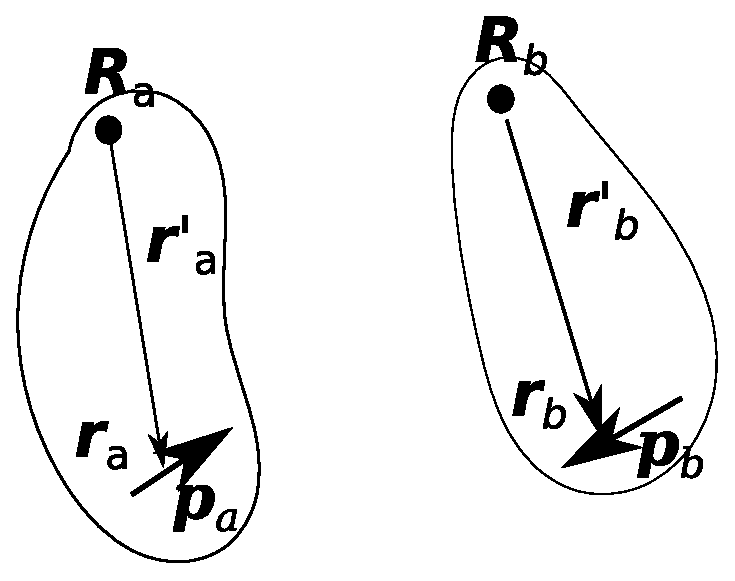
\includegraphics[clip,width=0.6\linewidth]{pict/3_3_3_dipoles.eps}
  \caption{ 磁気ダイポールの相互作用。位置$\bm{r}_a=\bm{R}_a+\bm{r}'_a$と$\bm{r}_b=\bm{R}_b+\bm{r}'_b$に磁気ダイポール$\bm{p}_a$および$\bm{p}_b$がある。}
  \label{fig:3_3_3_dipoles}
\end{figure}
図\ref{fig:3_3_3_dipoles}のように、2つの剛体に位置$\bm{r}_a$と$\bm{r}_b$に磁気ダイポール$\bm{p}_a$と$\bm{p}_b$の相互作用を考える。

位置$\bm{r}_a$は、回転の中心のベクトル$\bm{R}_a$と回転からの中心から磁気ダイポールまでのベクトルを$\bm{r}'_a$とする。すなわち$\bm{r}_a=\bm{R}_a+\bm{r}'_a$である。
また、$\bm{r}'_a$および$\bm{p}_a$は、剛体$a$の向き$\bm{u}_{a1},\bm{u}_{a2},\bm{u}_{a3}$に依存する。
\begin{equation}
\bm{r}_a=\bm{R}_a+\sum_{i=1,2,3}r'_{ai}\bm{u}_{ai}
\end{equation}
\begin{equation}
\bm{p}_a=\sum_{i=1,2,3}p_{ai}\bm{u}_{ai}
\end{equation}
と書くと便利である。
また、剛体$b$に関しても同様であるし、剛体に複数のダイポールがある場合に拡張は容易である。

2つの磁気ダイポール$\bm{p}_a, \bm{p}_b$の相互作用によるポテンシャルエネルギー$U$は、以下のとおりである。
\begin{equation}
U=-\frac{\mu_0}{4\pi r_{ab}^3}\left(3\frac{\bm{r}_{ab}\bm{r}_{ab}}{r_{ab}^2}-\bm{\delta}\right):\left(\bm{p}_a\bm{p}_b\right)
\end{equation}
ここで$\mu_0$は透磁率で
\begin{eqnarray}
\bm{r}_{ab}&=&\bm{r}_b-\bm{r}_a\nonumber\\
&=&\bm{R}_b+\sum_ir'_{bi}\bm{u}_{bi}-\bm{R}_a-\sum_ir'_{ai}\bm{u}_{ai}
\end{eqnarray}
である。
剛体$a$に働くトルク$\bm{T}_a$は、
\begin{eqnarray}
\bm{T}_a&=&-\vecR_a U\nonumber\\
&=&-(\vecR_a\bm{r}_{ab})\cdot\frac{\partial U}{\partial \bm{r}_{ab}}-(\vecR_a\bm{p}_{a})\cdot\frac{\partial U}{\partial \bm{p}_{a}}
\end{eqnarray}
で計算される。ここで
\begin{equation}
\vecR_a=\sum_{i=1,2,3}\bm{u}_{ai}\times\frac{\partial}{\partial \bm{u}_{ai}}
\end{equation}
である。
\begin{equation}
\frac{\partial U}{\partial \bm{r}_{ab}}=-\frac{3\mu_0}{4\pi r_{ab}^5}
\left(-5\frac{(\bm{r}_{ab}\cdot\bm{p}_a)(\bm{r}_{ab}\cdot\bm{p}_b)\bm{r}_{ab}}{r_{ab}^2}
+(\bm{p}_b\cdot\bm{r}_{ab})\bm{p}_a
+(\bm{p}_a\cdot\bm{r}_{ab})\bm{p}_b
+(\bm{p}_a\cdot\bm{p}_{b})\bm{r}_{ab}
\right)
\end{equation}
\begin{equation}
\frac{\partial U}{\partial \bm{p}_a}=-\frac{\mu_0}{4\pi r_{ab}^3}\left(3\frac{(\bm{r}_{ab}\bm{p}_b)\bm{r}_{ab}}{r_{ab}^2}-\bm{p}_b\right)
\end{equation}
\begin{equation}
\R_{a\alpha}r_{ab\beta}=-\sum_ie_{\alpha\gamma\beta}u_{ai\gamma}r'_{ai}
\end{equation}
\begin{equation}
\R_{a\alpha}p_{ab\beta}=\sum_ie_{\alpha\gamma\beta}u_{ai\gamma}p_{ai}
\end{equation}
と計算されることから、
\begin{equation}
\bm{T}_a=-\vecR_a U=\bm{r}'_a\times\frac{\partial U}{\partial \bm{r}_{ab}}
-\bm{p}_a\times\frac{\partial U}{\partial \bm{p}_{a}}
\end{equation}
となる。
%%%%%%%%%%%%%%%%%%%%%%%%%%%%%%%%%%%%%%%
\chapter{シミュレーション方法}
 %%%%%%%%%%%%%%%%%%%%%%%%%%%%%%%%
 \section{慣性モーメント}
 剛体の回転運動を計算する前に、剛体の慣性モーメントテンソルを見積もる必要がある。
 図\ref{fig:4_1_inertia}(c)の形の剛体の慣性モーメントテンソルを(a),(b)と計算して(c)を見積もる。
 (a)では、慣性モーメントテンソルを式\eqref{eq:inertia_sphere}および式\eqref{eq:inertia_cylinder}から見積もる。
 ここでは、重心のまわりでの慣性モーメントテンソルとなる。
 (b)で、平行移動の公式\eqref{eq:steiner}を用いて目的の回転中心に移動した慣性モーメントテンソルを求める。
 (c)で、2つの慣性モーメントを足し合わせて目的の慣性モーメントテンソルとなる。
 \begin{figure}[h]
\centering
  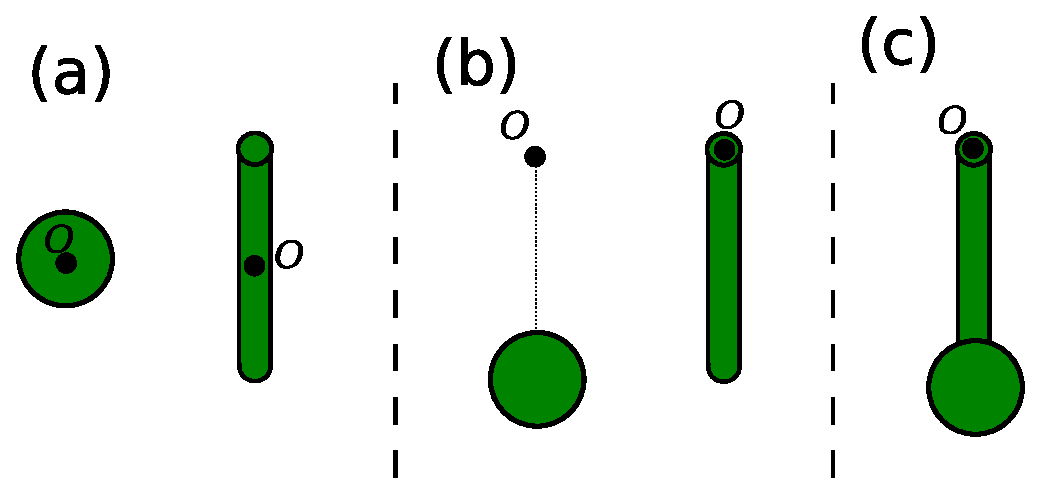
\includegraphics[clip,width=0.75\linewidth]{pict/4_1_inertia.eps}
  \caption{慣性モーメントテンソルの評価。(a)それぞれの重心のまわりで慣性モーメントテンソルを計算。
  (b)平行移動の定理で平行移動した後のテンソルを評価。(c)平行移動したテンソルを足し合わせる。}
  \label{fig:4_1_inertia}
\end{figure}

式\eqref{eq:omega}で、慣性モーメントテンソルの逆行列を計算するが必要がある。
ただし、たとえば、大きさのない質点からなる振り子などでは、固有値がゼロになる場合があり、逆行列が計算できない。
慣性モーメントテンソルをスペクトル分解して、
\begin{equation}
\bm{I}=\sum_{i=1,2,3}\lambda_i\bm{n}_i\bm{n}_i
\end{equation}
と出来る。ここで、$\lambda_i$は、固有値で、$\bm{n}_i$そのときの単位固有ベクトルが$\bm{n}_i$である。
逆行列の計算は、
\begin{equation}
\bm{I}^{-1}=\sum_{\lambda_i\neq 0}\frac{1}{\lambda_i}\bm{n}_i\bm{n}_i
\end{equation}
と固有値がゼロの場合を除いて計算する。
 \section{時間積分}
 時間$t$の剛体の向きから、時間$t+\Delta t$の剛体の向きを計算する。
\subsection{オイラー法}
式\eqref{eq:dLdt}を差分で
\begin{equation}
\bm{L}(t+\Delta t)=\bm{L}(t)+\bm{T}(t)\Delta t
\end{equation}
と計算する。式\eqref{eq:omega}から、角速度$\bm{\omega}(t)$を計算する。
式\eqref{eq:dudt}から、
\begin{equation}
\bm{u}_i(t+\Delta t)=\bm{u}_i(t)+\bm{\omega}(t)\times\bm{u}_i(t)\Delta t
\end{equation}
となる。
このように時間発展を計算することで、剛体の向き$\bm{u}_i$を計算できる。
\subsection{4次のルンゲクッタ法}
先のオイラー法では、十分な計算精度を確保するために、$\Delta t$の値を小さくする必要がある。
そのため、ここでは、4次のルンゲクッタ法で計算する方法を述べる。
$t^1=t$として、
\begin{equation}
\bm{T}^1=\bm{T}(t^1), \quad \bm{\omega}_1=\bm{\omega}(t^1),\quad \bm{u}_i^1=\bm{u}_i(t^1)
\end{equation}
とする。
次に
\begin{equation}
\Delta \bm{L}^1=\bm{T}^1\Delta t, \quad \Delta\bm{u}_i^1=(\bm{\omega}^1\times\bm{u}_i^1)\Delta t
\end{equation}
\begin{equation}
\bm{L}^2=\bm{L}^1+\frac12\Delta \bm{L}^1,\quad\bm{u}_i^2=\bm{u}_i^1+\frac12\Delta\bm{u}_i^1
\end{equation}
\begin{equation}
 \bm{\omega}^2=\sum_{i,j=1,2,3}(I^{-1})_{ij}\bm{L}^2\cdot\bm{u}_i^2\bm{u}_j^2
\end{equation}
と計算する。これらから、$t^2=t^1+\Delta t/2$のトルク$\bm{T}^2$を計算する。同様に
\begin{equation}
\Delta \bm{L}^2=\bm{T}^2\Delta t, \quad \Delta\bm{u}_i^2=(\bm{\omega}^2\times\bm{u}_i^2)\Delta t
\end{equation}
\begin{equation}
\bm{L}^3=\bm{L}^1+\frac12\Delta \bm{L}^2,\quad\bm{u}_i^3=\bm{u}_i^1+\frac12\Delta\bm{u}_i^2
\end{equation}
\begin{equation}
 \bm{\omega}^3=\sum_{i,j=1,2,3}(I^{-1})_{ij}\bm{L}^3\cdot\bm{u}_i^3\bm{u}_j^3
\end{equation}
と計算する。また、$t^3=t^1+\Delta t/2$として、トルク$\bm{T}^3$を計算する。さらに、
\begin{equation}
\Delta \bm{L}^3=\bm{T}^3\Delta t, \quad \Delta\bm{u}_i^3=(\bm{\omega}^3\times\bm{u}_i^3)\Delta t
\end{equation}
\begin{equation}
\bm{L}^4=\bm{L}^1+\Delta \bm{L}^3,\quad\bm{u}_i^4=\bm{u}_i^1+\Delta\bm{u}_i^3
\end{equation}
\begin{equation}
 \bm{\omega}^4=\sum_{i,j=1,2,3}(I^{-1})_{ij}\bm{L}^4\cdot\bm{u}_i^4\bm{u}_j^4
\end{equation}
これから、やはりトルク$\bm{T}^4$を計算する。
\begin{equation}
\Delta \bm{L}^4=\bm{T}^4\Delta t, \quad \Delta\bm{u}_i^4=(\bm{\omega}^4\times\bm{u}_i^4)\Delta t
\end{equation}
これらから、
\begin{equation}
\bm{L}(t+\Delta t)=\bm{L}^1+\frac16(\Delta\bm{L}^1+2\Delta\bm{L}^2+2\Delta\bm{L}^3+\Delta\bm{L}^4)
\end{equation}
\begin{equation}
\bm{u}_i(t+\Delta t)=\bm{u}_i^1+\frac16(\Delta\bm{u}_i^1+2\Delta\bm{u}_i^2+2\Delta\bm{u}_i^3+\Delta\bm{u}_i^4)
\end{equation}
\begin{equation}
 \bm{\omega}(t+\Delta t)=\sum_{i,j=1,2,3}(I^{-1})_{ij}\bm{L}(t+\Delta t)\cdot\bm{u}_i(t+\Delta t)\bm{u}_j(t+\Delta t)
\end{equation}
と計算する。
 %%%%%%%%%%%%%%%%%%%%%%%%%%%%%%%%
 \chapter{操作例}
 %%%%%%%%%%%%%%%%%%%%%%%%%%%%%%
\chapter{UDF説明}
\chapter{action 説明}
\chapter{Python説明}
 
  \end{document}

